\section{Evaluation}
In this section, we show the feasibility of the approach of using declarative
dataflow analysis for multilingual program, and the effectiveness of its
implentation. More specifically, we set three RQs as follow: RQ1) Feasibility:
Is the approach of declarative dataflow analysis for multilingual program
fesible?  RQ2) Performance: How is the spped and precision of analyzer,
compared to the previous approach?  RQ3) Usefulness: How practical is the
analyzer?  To answer RQ1, we ran our analyzer to NativeFlowBench, a jni program
dataflow analysis benchmark.  NativeFlowBench is a set of 23 android
application featuring various interactions between C++ and Java, where some
applications contain a code that leaks sensitive user data by logging it.  To
answer RQ2 and RQ3, we ran our analyzer to 43 real-world applications collected
from F-Droid, a open-source application repository. We compared our analyzer
with state-of-the-art JNI analyzer, and show that our analyzer outperforms in
terms of speed and precision. We also found 28 interoperation bugs, including
20 newly found bugs.


\subsection{RQ1: Feasibility}
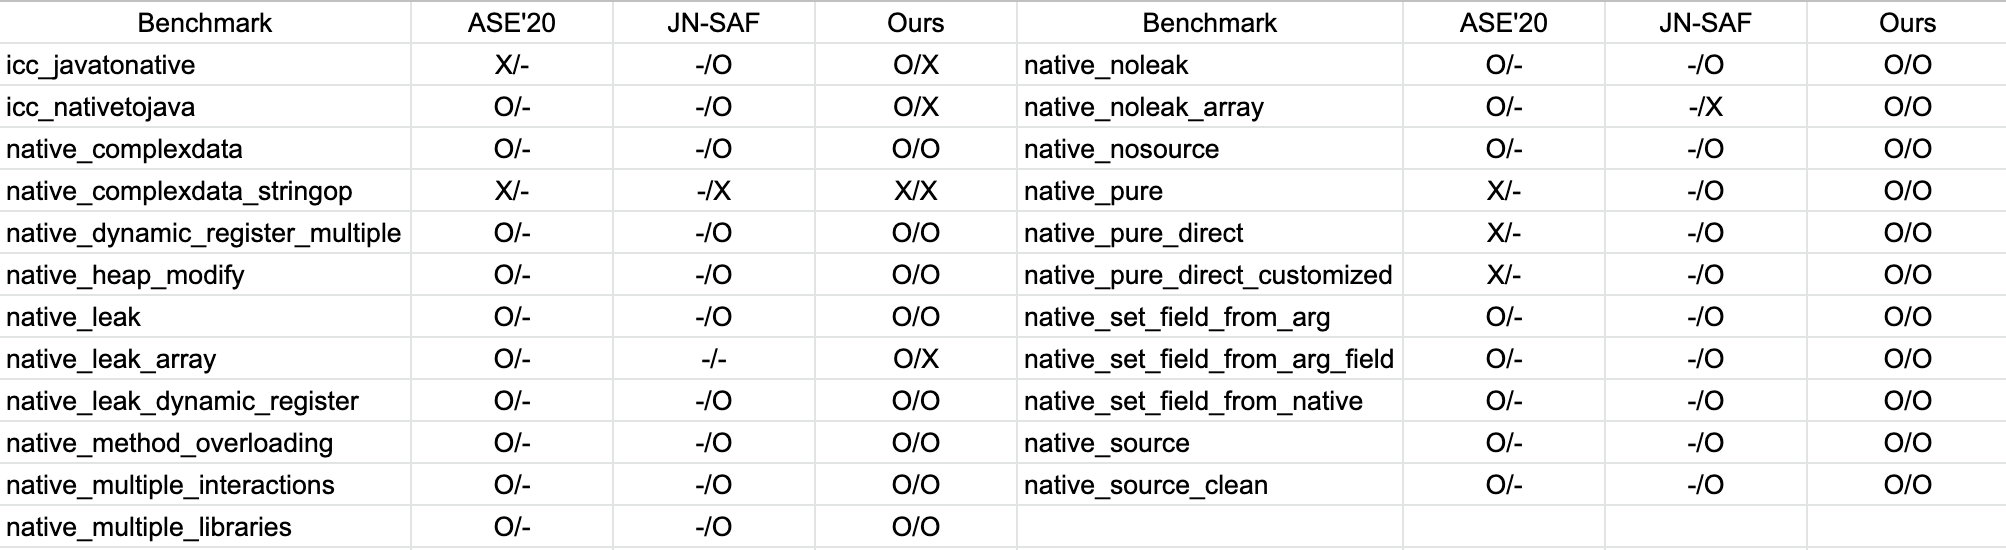
\includegraphics[width=0.5\textwidth]{img/table1}
The table1 shows the analysis result for 19 benchmarks in NativeFlowBench.  The
"Benchmark" coulmns denote the benchmark names, and "result" coulmns denote
whether the analysis result for corresponding benchmark was correct(O) or
not(X). We call that the analysis result is successful if every function call
target (call(j->c), call(c->j)) and field access tagret (field\_read(c->j),
field\_write(c->j)) are precisely determined, and every data leak is reported
correctly without false positives or false negatives.  The result shows that
except for one benchmark, our analyzer could correctly determine all targets
for function calls and field access correctly, and could successfully perform
dataflow analysis to find all of the data leaks. The only exception was
native\_compexdata\_stringop, where string manipulations functions such as
strcpy or strcat was used, and since the inner-flow analysis could not
properly handle these functions, analyzer could not correctly deterimine the
function call target.

\subsection{RQ2: Performance}
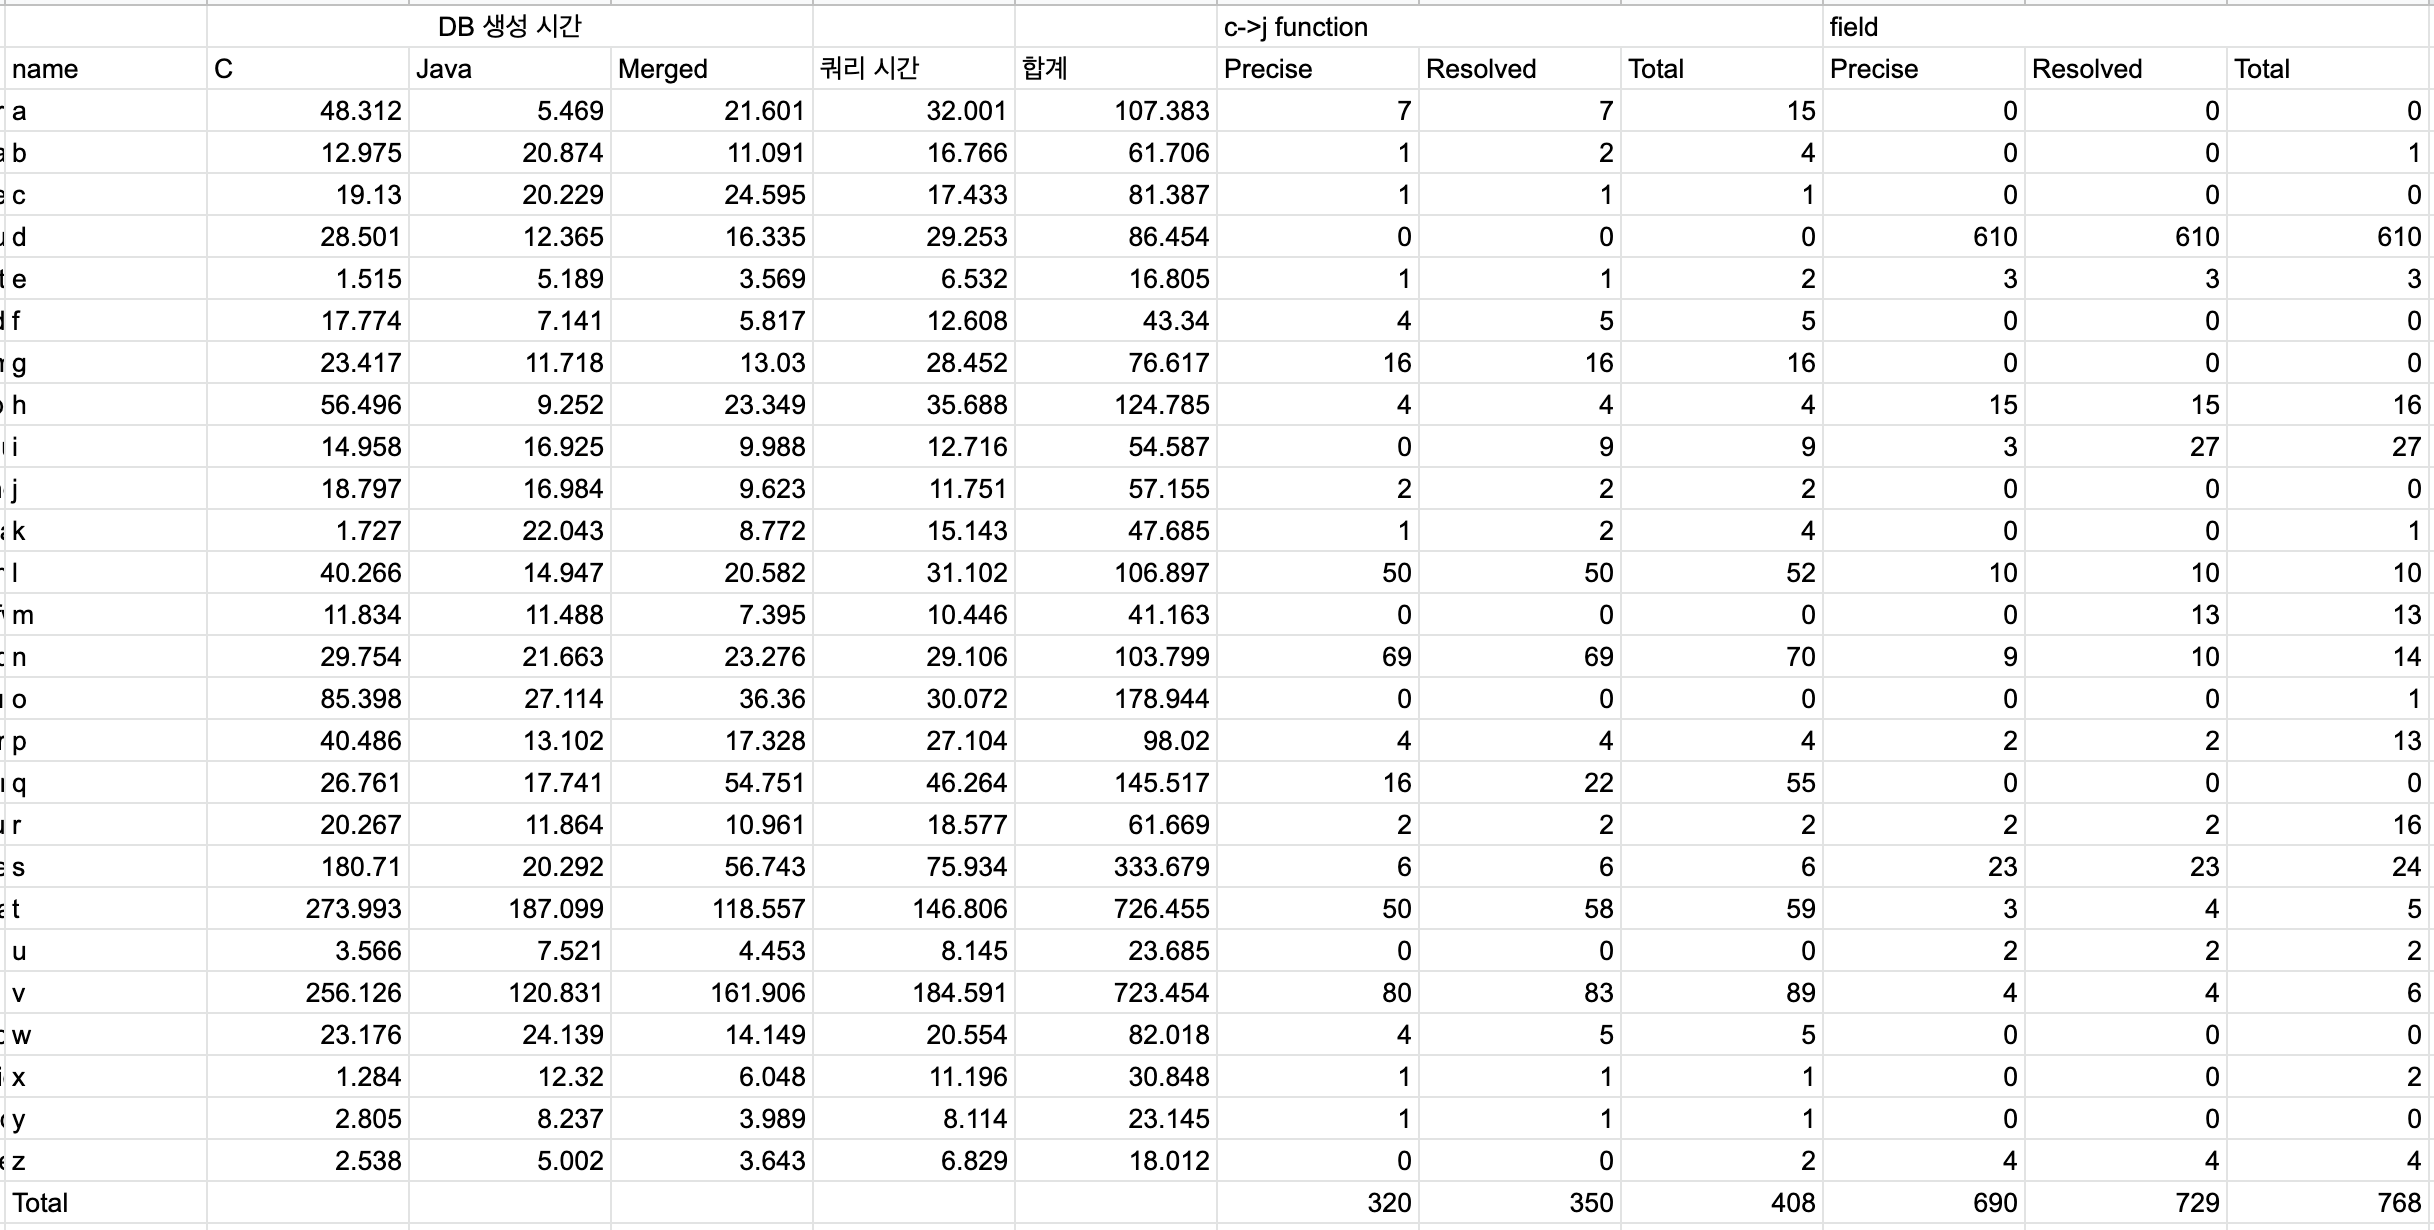
\includegraphics[width=0.5\textwidth]{img/table2}
The table2 shows the analysis result for 43 F-Droid applications. The "time" coulmn denotes
the time for creating database and evaluating query. The average time for creating DB was
??? seconds, and average time for evaluating query was ??? seconds, making the total analysis time
??? seconds. This is x4 faster on average, compared to the state-of-the art JNI program analyzer.
Note that time for creating DB includes compile time, and once DB is created, multiple queries can
be evaluated withou creating DB again. This means that pratically, the pratical speed up becomes x14.

The "precision" coulms denotes the precision of dispatching function call target, and field access target.
"Precise" means exactly one target was found, and resolved means at least one target was found.
Compared to the previous result, the precision was also higher for both function call targets and field access targets.

\subsection{RQ3: Usefulness}

